\part{Peuples}

\chapter{Humain}

\begin{multicols}{2}

\begin{center}
	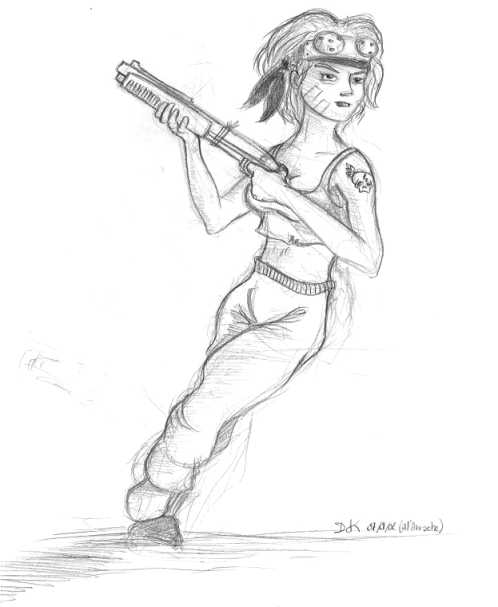
\includegraphics[width=123pt]{Img/humain}
\end{center}

\section{Physique}

En à peine un siècle, le corps humain n'a pas radicalement évolué. Toutefois nous pouvons noter quelques petits changements intervenus dans la physionomie des humains selon leur habitat d'origine. Les humains ayant vécu principalement dans l'espace ou dans une planète à faible densité (notamment lors de leur croissance) sont globalement plus grands (moyenne 1m77). Leurs corps sont plus élancés devenant alors bien plus propices aux déplacements souples et acrobatiques nécessaires à la vie dans l'espace, qu'aux efforts musculaires intenses. Inversement, ceux ayant vécu sur une planète ayant une densité supérieure à celle de la terre sont souvent plus petits (moyenne 1m55), plus trapus, et plus costauds. Cette évolution n'est toutefois pas suffisamment présente pour créer une véritable marque distinctive. Globalement, le corps humain s'adapte à ces différents milieux de vie. Humains :Mais cette évolution est lente et n'est pas encore arrivée à son terme.

\section{Culture}

Dans la théorie, les nations humaines sont regroupées sous la bannière de l'alliance Terrienne, une alliance puissante, unifiée, capable de faire face à l'adversité. Grâce à l'alliance Terrienne, les humains sont enfin capables de faire front commun vis à vis des autres peuples. Dans la théorie...

Dans la pratique, malheureusement, l'alliance Terienne ne fonctionne correctement qu'en cas de crise. Le reste du temps, elle est une façade derrière laquelle se trouve encore 4 grandes nations, 4 grands blocs indépendants :
\begin{itemize}
	\item l'Alliance Américaine qui regroupe l'Amérique du nord et l'Amérique du sud.
	\item la Fédération Européenne contenant l'Europe et les pays au bord de la méditerranée. 
	\item l'Empire d'Orient, qui contient la chine ainsi que le Japon.
	\item l'Union Africaine
\end{itemize}

L'Union Africaine n'a que peu de moyen et de pouvoir. Pauvre, elle essaye désespérément de se sortir de sa misérable situation. On raconte que l'Union Africaine soutient secrètement plusieurs clans pirates, échangeant du matériel contre du ravitaillement et les richesses adverses. Certaines rumeurs accusent également l'Union Africaine de cacher une partie de ses forces armées parmis ces pirates... 

Autrefois, la Fédération Européenne était une des puissances phares Teriennes. Présente sur le plan diplomatique et politique, elle était très engagée dans la Deneb, profitant de ses complexes rouages pour améliorer sa situation. La chute de celle-ci a porté un coup sévère à l'Europe. Aujourd'hui, celle-ci s'est fait plus discrète. Pour certains, l'Europe essaye actuellement de se faire oublier dans l'espoir que les autres nations Terriennes ne profitent de la situation actuelle pour se venger de nombreux coups tordus qu'elle a pu porter.

L'alliance Américaine est en réalité dirigée par une poignée de méga-corporations. Le gouvernement officiel est tellement corrompu et affaibli qu'ils n'ont plus aucun pouvoir sur leur propre politique. Toutefois, depuis la fondation du Bureau Corporatiste, ces méga-corporations se retrouvent dans une situation délicate. Engagées dans l'alliance Terienne, elles ne peuvent pas officiellement s'allier au Bureau Corporatiste. Cette décision ne serait pas comprise par le peuple Terrien. Séparées du Bureau Corporatiste, elles perdent par contre un fort pouvoir commercialeet perdent donc de leur influence au niveau Galactique. Les corporations Américaines sont donc obligées de jouer à un jeu dangereux.

L'empire d'Orient est aujourd'hui la nation terrienne la plus puissante et la plus stable. Il s'agit d'un empire autoritaire fortement militarisé. Il représente la véritable force de frappe Humaine. Actuellement, l'alliance Terrienne est en guerre contre le Protectorat Teldrim. Dans les faits, ce sont principalement les forces de l'empire qui sont engagées. D'une manière générale, les habitants de l'empire sont extrêmement Xénophobes.

\section{La Religion}

Plusieurs religions terriennes ont survécu a travers les âges mais les plus pratiquées restent deux religions monothéistes : le Christianisme et l'Islamisme. Le bouddhisme, dans son expression philosophique, a également survécu et s'est vu doté d'un nouvel élan mystique, incorporant à ces croyances certains éléments du Shintoïsme. Même si elles sont très présentes, les religions gardent, au niveau humain, un poids politique assez faible.

\section{Ce qu'ils pensent des ...}

\begin{itemize}
\item Centauriens : Ils se sont laissés corrompre par les Ergios. Un jour ils comprendront qu'ils sont toujours humains.
\item Snagirs : Ces lézards arrogants pensent que rien ne peu les atteindre mais ils se trompent ! Avec leurs grands airs ils refusent de se mêler aux conflits des autres peuples, mais un jour ils devront faire face à leurs responsabilités.
\item Teldrims : Des chats enragés qu'ils nous faut mater. Quand le peuple Teldrim aura apprit à rejeter sa stupide foi, nous pourrons discuter avec eux plus sainement.
\item Vélïos fédéraux : Ce sont des frères d'armes, de potentiels alliés. Ils savent où est leurs forces et l'usent avec intelligence. Nous regrettons qu'ils soient si peu nombreux.
\item Vélïos impériaux : Nous ne les comprenons pas, ils ont abandonnés les mondes fédéraux sans explication. Je crois que nous devons nous méfier de leurs impératrices.
\item Nomades : Des hors-la-loi, des exilés, ce qui se fait de pire dans chacun de nos peuples. Ils ont décidé de s'occuper des tâches ingrates... Pourquoi pas ? Prenons ça comme une sorte de réinsertion.
\end{itemize}

\end{multicols}

\regle{Création de personnages Humains}{
Lors de la création, les personnages Humains démarrent le jeu avec le trait suivant : 
\begin{itemize}
\item Sens de la tromperie (Social)
\end{itemize}
}

\chapter{Centauriens}

\begin{multicols}{2}

\begin{center}
	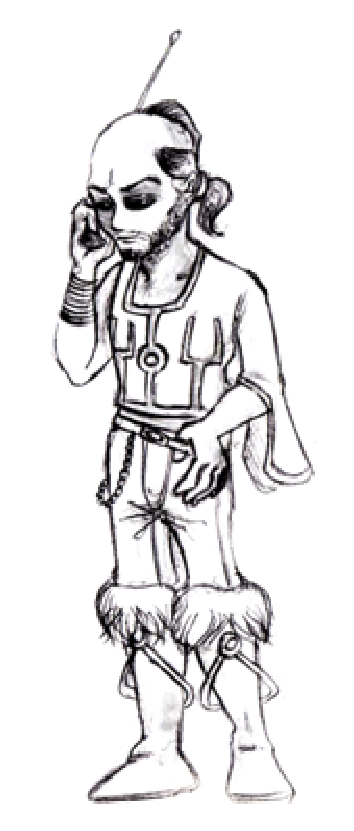
\includegraphics[scale=0.5]{Img/centaurien}
\end{center}

\section{Physique}

L'aspect des Centauriens est encore assez similaire à celui des humains dont ils sont les descendants. Toutefois, la vie sur Alpha Centauri a provoqué chez eux une évolution spectaculaire. À peine un siècle après leur arrivée, les Centauriens avaient déjà subi toutes les mutations qu'on leur connait aujourd'hui. On suspecte des radiations originaires de leurs deux soleils d'être responsables de cette évolution rapide. Humains :

Les Centauriens sont plus petits que les humains. Ils mesurent en moyenne 1m49 pour un poids moyens de 40 Kg. Malgré leur taille et leur poids, ils n'en gardent pas moins des traits adultes et ne peuvent pas être confondus avec des enfants humains. 

Leurs yeux portent l'une de leurs mutations majeures. Leur iris s'est totalement dilaté et recouvre maintenant l'intégralité de l'œil. Leurs yeux peuvent prendre des couleurs similaires à ceux des humains.

La peau des Centauriens est devenue sombre et terne, sans prendre toutefois la teinte brune de la population Africaine. Au contraire leur peau est maintenant gris-cendre. Leur couleur de peau leur vaut l'appellation de "petits Gris" chez les humains. Une appellation raciste chargée de mépris. 

\section{Culture}

L'origine des Centauriens remonte au programme de colonisation Américain : Nouveaux Mondes. Lors de ce programme, les Humains ont envoyé 15 000 colons dans l'espace en direction de plusieurs étoiles dont Alpha Centauri. Des vaisseaux générations, des vaisseaux stases, ... Des vaisseaux de tous types furent envoyés à travers les étoiles. Les scientifiques terriens avaient largement surestimé la résistance et la qualité du matériel composant les vaisseaux. Très vite ceux-ci commencèrent à montrer des défaillances. La situation semblait désespérée quand des vaisseaux Ergios sont venus porter secours aux colons Terriens. Les Ergios transportèrent les humains survivants jusqu'à Centauri. Ils leurs portèrent l'assistance nécessaire à la fondation de la colonie. Il ne restait toutefois plus que 10 000 colons. On estime l'intervention Ergios à environ 5 ans après le début du projet. 

Les Centauri ont fortement été marqués par cet épisode.

Ils ont tout d'abord hérité d'un grand respect envers les Ergios qu'ils considéraient, et considèrent toujours comme leurs sauveurs. Durant la guerre ils se sont d'ailleurs rangés du coté de ces derniers. Cette acte à failli leur coûter très cher lors de l'exil Ergios. Il a fallu une intervention diplomatique et militaire Snagir pour que les Centauriens soient laissés en paix et même intégrés à la fédération ! Humains :

Deuxièmement, durant leur installation ils ont beaucoup profité de l'aide Ergios. Leur planète natale porte encore des nombreuses traces de leur technologie. Les Centauriens sont sûrement ceux qui la connaisse et la comprenne le mieux. Les Ergios ne leur ont toutefois jamais appris à la reproduire. Actuellement la population Centaurienne s'élève à 30 000 personnes.

La famille est au centre même de l'organisation Centaurienne. Les parents Centauriens ont en moyenne 5 enfants. 

Les Centauriens font front derrière le conseil des « Gardiens » et leurs élus, le Brash'Rack. Le Brash'Rack correspond au gouvernement Centaurien, ou à ce qui s'en rapproche le plus. 

L'intégralité des Centauriens possède un lien Télépathique entre eux, canalisé par le cristal d'Agavas. Le Brash'Rack a la charge de protéger le cristal dans la capitale. Ce lien télépathique est le seul moyen connu de communication instantané entre deux points éloignés dans l'univers.

Les Centauriens sont donc extrêmement prisés pour leurs talents spéciaux par les différentes organisations de la Deneb. Ce peuple reste toutefois très renfermé sur lui-même et le Brash'Rack surveille de près l'usage de la Télépathie. 

\section{Religions}

Les Centauriens ont totalement abandonné les religions Terriennes et n'ont pas adopté de nouvelles croyances. Toutefois, leur vénération des Ergios et de leur savoir est telle qu'elle pourrait ressembler à une religion. Les Centauriens ne le voient pas ainsi. Ils savent que les Ergios ne sont pas des dieux, mais simplement des êtres à la technologie évoluée.

\section{Ce qu'ils pensent des ...}

\begin{itemize}
\item Humains : Malheureusement les Ergios n'ont pas pu ouvrir les yeux de nos frères. C'est à nous qu'incombe maintenant cette lourde tâche.
\item Snagirs : Un peuple sage qui ne se laisse pas dominer par ses pulsions. Nous craignons toutefois qu'ils cachent des secrets peu reluisants.
\item Teldrims : Un peuple jeune qui ne sais pas refréner leurs ardeurs. Leurs religions est la seule chose qui les tempèrent un peu et doit être maintenus coute que coute.
\item Vélïos fédéraux : Leurs grandes forces les as rendus calme et sûr d'eux. Les Vélïos sont nos meilleurs alliés et je pense que nous leurs devons d'être encore en vie.
\item Vélïos impériaux : Quels secrets cachent l'impératrice pour s'être repliés ainsi. Si les Vélïos ne se révoltent par contre elle, nous craignons pour la suite.
\item Nomades : La vie est difficile dans les étoiles, les nomades ont appris à se serrer les coudes sans distinction de races. Si seulement d'autres peuples pouvaient en tirer une leçon...
\end{itemize}

\end{multicols}

\regle{Création de personnage Centauriens}{
Lors de la création, les personnages Centauriens démarrent le jeu avec le trait suivant : 

\begin{itemize}
\item Lien Centaurien (Télépathie)
\end{itemize}
}

\chapter{Snagir}

\begin{multicols}{2}

\begin{center}
	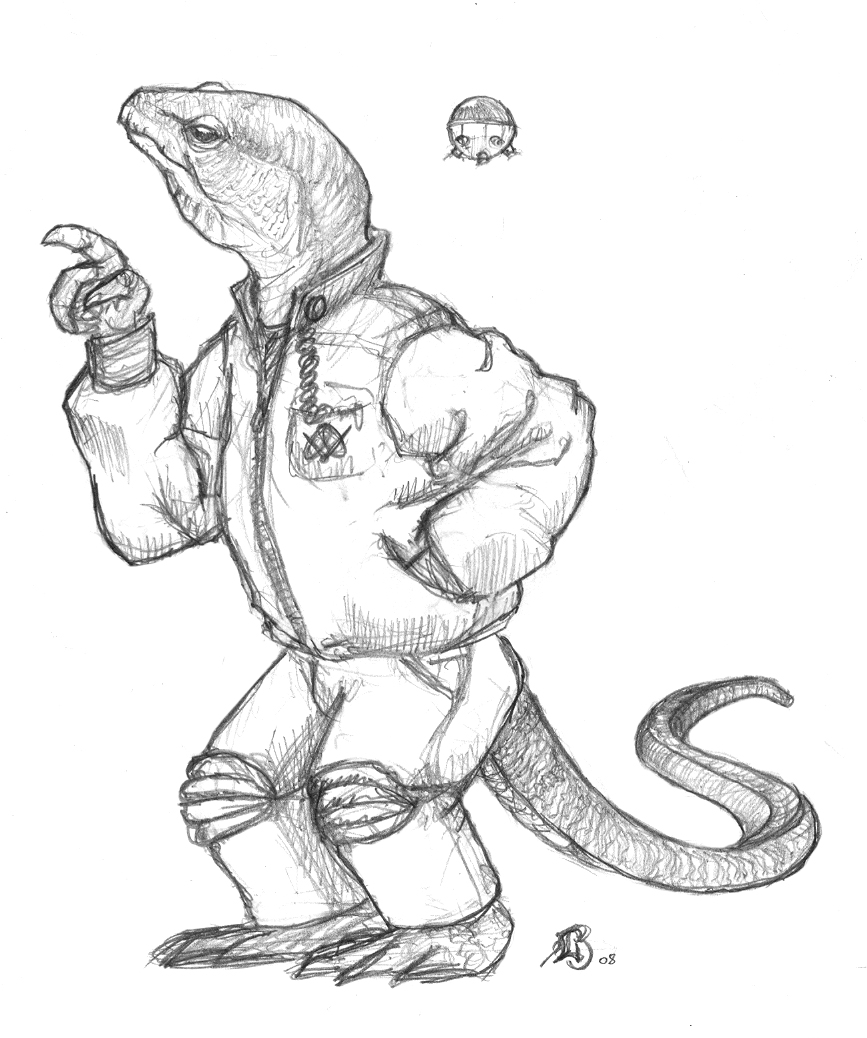
\includegraphics[width=143pt]{Img/snagir}
\end{center}

\section{Physique}

Comme toutes les races de la fédération, les Snagirs sont des humanoïdes bipèdes. Ils ont toutefois la particularité d'être aussi à l'aise sur leur deux jambes postérieures, qu'en utilisant leurs quatre membres.

La seconde particularité des Snagirs est leur mode respiratoire : ils sont dotés de la respiration cutanée en plus de poumons. Ils sont donc capables de respirer sous l'eau comme en dehors. Le milieu aquatique fut autrefois leur milieu de prédilection, même si leurs cités sous-marines sont maintenant isolées.

En dehors de ça, la race Snagir est la plus petite de la Fédération, mesurant en moyenne 1m30. Leur peau est recouverte d'écailles et peut prendre diverses teintes selon leur milieu d'origine : vert, orange, ou marron. Leur visage est anguleux et totalement dépourvu d'oreille. 

Leur corps se termine par une longue queue n'ayant d'autre utilité que l'amélioration de stabilité qu'elle leur confère. Cette appendice leur reste de leur passé, une époque où, selon certains scientifiques, ils utilisaient cette queue pour se défendre, et leurs coups auraient été redoutables. L'évolution Snagir l'a toutefois rendue totalement obsolète.

Les humains font souvent le parallèle entre les Snagirs et les reptiles terriens comme par exemple les dragons de Komodo. Des études effectuées par des savants Snagirs ont bien sûr démenti toute possibilité de parenté même lointaine.

\section{Natalité et espérance de vie}

Les Snagirs ont un taux de reproduction extrêmement faible. Rares sont les couples qui auront plus de 2 enfants. Leur population a donc une forte tendance à la stagnation.

Par contre, les Snagirs ont unes espérance de vie moyenne de 300 ans. Certains Snagirs ont même réussi à atteindre l'âge exceptionnel de 500 ans ! 

Un Snagir est considéré adulte à partir du moment où il a passé le Sssack'Hisssh, l'épreuve « d'âge adulte ». Cette épreuve consiste simplement à apporter une innovation technologique (même mineure) qui sera validée par le conseil. 

\section{Culture}

Il y a peu, la société Snagir était encore fondée sur un système pyramidal très strict, très rigoureux. La Pyramide partait de l'échelon le plus proche, la famille, pour remonter jusqu'à l'Ambassadeur par diverses étapes : villages, clans, régions, planètes, ... Le système était alors démocratique, procédant par votes à chaque échelon. Le gouvernement était donc extrêmement long à prendre des décisions.

La prise de pouvoir réalisée par le Consortium est venue bouleverser cette méthode.

Le Consortium est organisé comme une société performante. La méthode est toujours pyramidale, mais le découpage se fait maintenant par domaine de compétences. Chaque personne de la pyramide a son domaine de responsabilité. Le Consortium attend de chacun qu'il prenne ses décisions. Plus question de votes, les décisions sont prises par un responsable. Le seul recours face à une décision est de consulter le supérieur de celui l'ayant prise.

Ce système est peut être moins fiable que l'ancien mode de gouvernement, mais il est bien plus réactif. Le Consortium, depuis son arrivée, a fait davantage évoluer les Snagirs que leur ancien gouvernement durant les trois derniers siècles.

Depuis l'arrivée du Consortium au pouvoir, les Snagirs sont devenus une force non négligeable dont chacun se méfie.

\section{Religion}

Les Snagirs sont antireligieux. Ils considèrent toute religion comme nuisible et contraire à leur esprit scientifique. La seule chose qui se rapproche d'une religion chez eux est leur croyance dans l'Esprit de la Machine. Toute machine, même la moins complexe, possède une âme qui lui est propre. Savoir parler à cette âme permet de devenir maître de l'objet et de sa technologie.

\section{Ce qu'ils pensent des ...}

\begin{itemize}
\item Humains : Ils ont un grand potentiel mais sont dévorés par leurs soifs de pouvoir. Tant pis pour eux, les Teldrims auront raisons d'eux.
\item Centauriens : Nous aimons ce peuple qui lutte pour sa survie. Dès qu'ils auront oubliés les Ergios ce seront nos meilleurs alliés.
\item Teldrims : Impulsifs, aveuglés par leurs religions, ils ne sont pas dignes de confiance. Heureusement ils sont facilement manipulable.
\item Vélïos fédéraux : Ils résolvent tous leurs conflits par la violence. Ce sont des brutes sans cervelles.
\item Vélïos impériaux : L'impératrice a été empreint d'une grande sagesse quand elle s'est retirée du combat. Elle n'aurait toutefois jamais du reprendre contact avec les mondes fédéraux.
\item Nomades : Ils partagent notre fascination et notre respect pour les machines. Peut-être pourrons-nous leur faire comprendre et entendre les esprits.
\end{itemize}

\end{multicols}

\regle{Création de personnage Snagir}{
Lors de la création, les personnages Snagirs démarrent le jeu avec le trait suivant : 
\begin{itemize}
\item Esprit de la machine (Intellect)
\end{itemize}
}

\chapter{Teldrim}

\begin{multicols}{2}

\begin{center}
	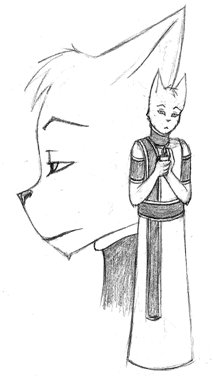
\includegraphics[width=113pt]{Img/teldrim}
\end{center}

\section{Physique}

Humanoïde bipède de taille légèrement inférieure aux humains (en moyenne 1m55), leur peau est recouverte d'une fourrure à poils courts qui peut aller du gris clair jusqu'au noir en passant par des teintes bleutées, parfois unie et parfois rayée ou dégradée.

Ils possèdent deux oreilles légèrement pointues et de petits yeux ayant souvent une teinte orangée. Leurs doigts sont munis de griffes rétractiles.

Les Teldrims sont réputés pour leur grande agilité et leur aptitude au déplacement silencieux. Leur allure générale n'est pas sans rappeler les félins que l'on peut trouver sur la planète Terre, les humains utilisent d'ailleurs souvent cette comparaison dans leurs moqueries…

\section{Natalité et espérance de vie}

Les Teldrims sont le peuple ayant le taux de natalité le plus élevé mais aussi l'espérance de vie la plus courte. En moyenne, un Teldrim a une espérance de vie de 40 ans. Un Teldrim peut espérer avoir 8 à 10 enfants. Un Teldrim est considéré adulte à partir de l'âge de 10 ans. Au-delà de 30 ans, un Teldrim est un ancien. 

Les Teldrims sont la seule race à ne pas avoir de notion de famille. Les couples Teldrims se font et défont rapidement, en fonction des envies. Pour eux, il n'y a rien de choquant à changer tous les jours de partenaire. Les enfants issus d'une union ne sont pas élevés par leurs parents, mais directement par la communauté (par les membres de leur espèce plus exactement). Humains : 

\section{Culture}

La société Teldrim est uniquement organisée sous la notion d'espèce. Chaque espèce possède ses propres spécificités et spécialités. De plus chaque espèce est également destinée à un type de métier précis. L'historique de leur planète ne présente pas la moindre trace de nations, leur peuple semble toujours avoir été uni. 

Toutefois, le terme uni n'est pas non plus ce qui correspond vraiment au peuple Teldrim. Chacune des espèces à son propre gouvernement, son propre dieu, et son propre représentant de droit divin : les prophètes. Seule l'entente entretenue par les prophètes permet de maintenir un semblant d'unité.

Les cinq espèces sont les suivantes :
\begin{itemize}
	\item Les E'Rinims, destinés aux métiers scientifiques.
	\item Les O'Isthrioths, formant le corps combattants de leur peuple.
	\item Les An'Velanims, spécialisés dans toutes les actions nécessitant de la discrétion et de l'astuce.
	\item Les E'Malinoths, fervents défenseurs de l'art et de l'artisanat sous toutes ses formes.
	\item La dernière espèce n'a pas de nom… Il s'agit d'une espèce d'esclaves qui n'ont aucun droit ni liberté. Cette espèce est la seule qui n'a pas de représentant, ni de dieu d'ailleurs…
\end{itemize}

Les noms des cinq espèces majeures correspondent au nom de leurs dieux, on parle ainsi du peuple d'O'Isthrioth, du peuple d'E'Rinim, … Ces quatre noms correspondent également aux noms des 4 lunes restantes gravitant autour de leur planète natale. Nul ne peut dire à l'heure actuelle si ce sont les dieux qui ont donné leur nom aux lunes, ou inversement. Quand à la dernière lune, ou ce qu'il en reste, nul n'a retenu son nom, et l'espèce qui y est lié n'en a plus non plus.

La société Teldrim est dans l'ensemble très figée, l'évolution au mérite est extrêmement rare, les Teldrims ne comprennent d'ailleurs pas ce principe. La diminution sociale est également très rare, mais peut arriver sur faute grave (les fautes très graves entraînent la mort). Les Teldrims sont les derniers à être entrés en rébellion contre les Ergios et leur aide a été précieuse dans la bataille.

Les Teldrims connaissent également un pouvoir psy depuis longtemps : la maîtrise du Tellien, leur bois sacré. Les Teldrims sont tous testés durant leur enfance pour savoir s'ils ont un potentiel dans ce domaine. La seule exception concerne les esclaves pour qui tout contact avec le Tellien est interdit. Les Teldrims qui ont un potentiel sont alors éduqués par la prêtrise et destinés à devenir, une fois adulte, prêtres à leur tour.

\section{Les Teldrims et l'histoire}

L'histoire est le centre de la culture des Teldrims. Chez eux, tout est affaire de traditions et de légendes. Car c'est sous forme de légendes que le peuple Teldrim garde une trace de son passé. Tous les évènements, anciens comme récents, sont irrémédiablement transformés en légendes qui vont rentrer dans la Grande Epopée Teldrim. 

Les prêtres sont les dépositaires de la Grande Epopée. Ils ont pour charge de la conserver et de la transmettre de génération en génération. Ils ont également pour fonction de conter aux autres membres de leur peuple les fabuleuses légendes afin que tous soit conscients du destin du peuple Teldrim. Tous les Teldrims ont un grand respect pour la prêtrise et la Grande Epopée qui est pour eux l'âme de leur peuple.

En dehors des légendes présentes dans l'épopée, les Teldrims n'ont pas de récit « objectif » de leur histoire ni de récit réellement daté. 

\section{Religions}

Les Teldrims suivent les voies d'une religion unique qui guide leur peuple. Chaque espèce Teldrim est guidée par un dieu gardien. La prêtrise, gardienne des coutumes et de l'histoire du peuple Teldrim, est également le représentant de leur dieu.

La société Teldrim est une véritable Théocratie. Aucune autre croyance n'est tolérée.

\section{Langage}

Les Teldrims ont un unique langage articulé qui est la langue des esclaves. Tous les Teldrims connaissent et pratiquent cette langue utilisée pour la communication entre espèces. Dans cette langue, seules les consonnes ont une réelle importance. Les voyelles sont rajoutés à la prononciation uniquement pour rendre le langage plus agréable. Un même mot peut donc être prononcé de multiples manières différentes.

La langue des esclaves Teldrims a été définie en tant que langue commune. Toutefois, une orthgraphe précise a été alors définie pour chaque mot, voyelles comprises.

Les différentes espèces Teldrims possèdent chacunes leur propre langage. Ces langages ne sont toutefois pas des langues articulées mais des languages corporels, prenant en compte des bruits, des postures, des gestes, et même le hérissement des poils. Il est difficile pour un Teldrim de reproduire le langage d'une autre espèce. C'est strictement impossible pour le membre d'un autre peuple. Seul les Teldrims esclaves n'ont pas leur propre langage corporel.

\section{Nom}

Les Teldrims possèdent deux noms :
\begin{itemize}
\item un nom complet
\item un nom usuel
\end{itemize}

Le nom complet d'un Teldrim est en général assez long. Il est composé de cette manière :
\begin{itemize}
\item les deux premières syllabes correspondent au nom de naissance. Il est donné par les parents en fonction du lieu et du moment de la naissance du Teldrim.
\item les deux syllabes suivantes illustrent le passage à l'age adulte.
\item les syllabes suivantes illustrent les évènements importants de la vie du Teldrim.
\item le nom de l'espèce du Teldrim est rajouté à la fin
\end{itemize}

Hormis les deux premières syllabes, toutes les syllabes suivantes doivent être décidées et données par un prêtre. Chaque couple de syllabes a un sens propre. Le sens est déterminé par la consonne de chaque syllabe. Par exemple, l/r symbolise une victoire guerrière en tant que combattant, alors que l/k indique une victoire en tant que stratège.

Le nom usuel d'un Teldrim correspond, soit à son nom de naissance, soit à son nom d'âge adulte. Les esclaves ne possèdent qu'un nom de naissance.

Les prêtres peuvent également décider de retirer tout ou partie de son nom à un Teldrim (hormis son nom de naissance). Il s'agit d'une sentence grave et déshonorante pour les Teldrims.

Vous pourriez donc obtenir les noms suivants (en gras, la partie usuel du nom).

\begin{itemize}
\item \textbf{Malek}'VaeKat'O'Malinoth
\item Ishak'\textbf{LiaKar}'O'Isthrioth
\item Tandek'\textbf{Vilaer}'Tarvin'An'Velanim
\item \textbf{Missia}'Valine'E'Rinims
\end{itemize}

\section{Ce qu'ils pensent des ...}

\begin{itemize}
\item Humains : Assoiffée de conquêtes, ils s'en sont prit à notre peuple. Ils paieront pour cela.
\item Centauriens : Ils ne sont ni nombreux, ni puissants. Pour nous les Centauriens sont négligeables.
\item Snagirs : Ils ont compris qu'il ne faut pas se frotter à nous. Nous pouvons vivre avec eux.
\item Vélïos fédéraux : Ils ont la force, nous avons l'agilité. Ensemble nous pourrions faire de grande choses.
\item Vélïos impériaux : Nous ne les aimons pas, que ces lâches restent chez eux !
\item Nomades : Ils se croient tous permis car ils vivent parmi les étoiles. Un jour nous leurs apprendrons que eux aussi doivent se soumettre.
\end{itemize}

\end{multicols}

\regle{Création de personnage Teldrims}{
Lors de la création, les personnages Teldrims démarrent le jeu avec le trait suivant : 
\begin{itemize}
\item Pas de Félin (Physique)
\end{itemize}
}

\chapter{Vélïos}

\begin{multicols}{2}

\begin{center}
	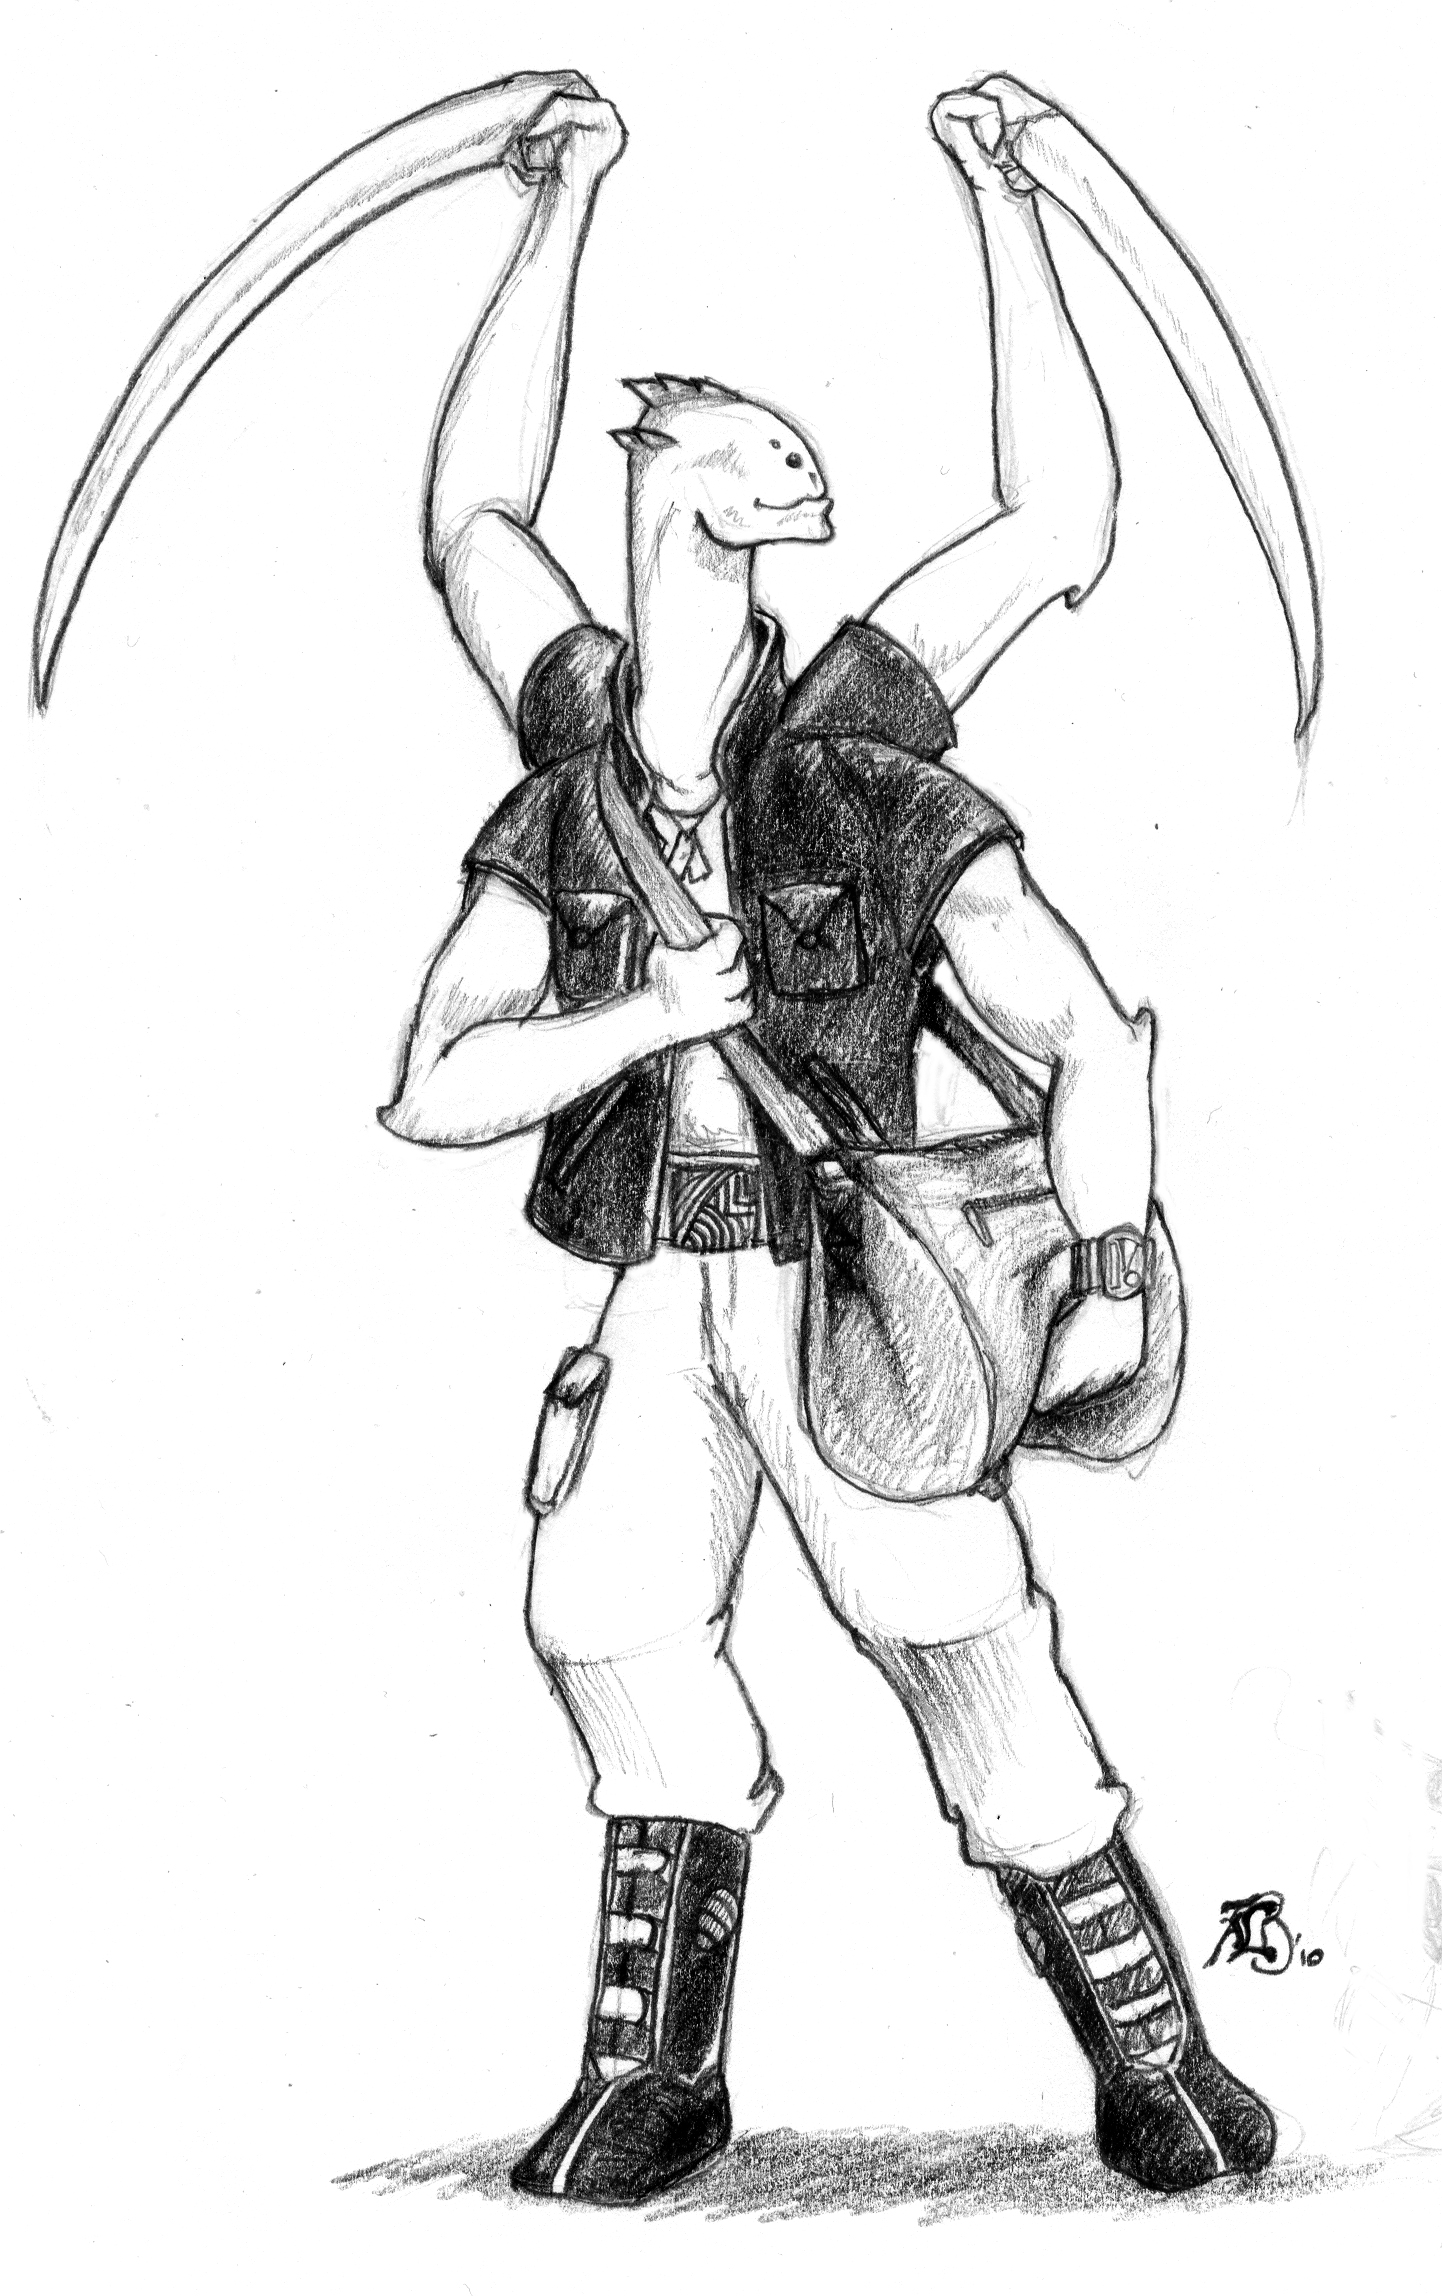
\includegraphics[width=123pt]{Img/velios}
\end{center}

\section{Physique}

Humanoïde bipède, les Vélïos sont les plus grands de la Fédération et mesurent en moyenne 1m93. Leur peau est de couleur très claire et prend en général des teintes bleues ou violettes. De premier abord, les Vélïos semblent être totalement imberbes. Toutefois leur corps est en fait revêtu d'un duvet de micropoils parcourant intégralement leur corps. 

Le système auditif des Vélïos passe par des appendices formant des sortes de crêtes sur leur crâne. Contrairement aux autres races qui possèdent des yeux à iris, les yeux des Vélïos sont constitués de multiples facettes, ressemblant aux yeux des araignées terriennes. 

Les Vélïos sont munis de deux grandes griffes dorsales. Ces griffes dorsales sont articulées à la base ainsi que dans leur milieu de façon à minimiser les mouvements nécessaires pour leur utilisation. Ces griffes forment des armes redoutables. Il s'agit sûrement d'une des raisons qui ont d'ailleurs incité le gouvernement fédéral à déclarer le port d'arme légal.

\section{Natalité et espérance de vie}

Les Vélïos ont une espérance de vie et un taux de natalité comparable à celui des humains.

\section{Culture}

Premier peuple allié aux humains, ce sont également les premiers à s'être retirés de la bataille ainsi que, au final, de la fédération galactique ! Lors de la guerre ce peuple au tempérament guerrier a mystérieusement décidé de s'isoler. Lors de cette retraite anticipée, la majeure partie de la population Vélïos a quitté les systèmes de la fédération. Aujourd'hui les Vélïos ayant décidé de rester sont totalement isolés de leur propre peuple. Il leur est maintenant impossible de revenir sur leur décision.

Avant la guerre galactique, le peuple Vélïos était régenté par un empire autoritaire. Selon des témoignages Vélïos, l'empereur était élu à vie suite à une série d'épreuves destinées à montrer sa force et son intelligence. Un nouvel empereur n'était alors élu qu'à la mort du précédent. Il semble toutefois qu'aucun empereur n'ait réussi à rester en vie plus d'une trentaine d'années.

Depuis leur départ, plus personne ne sait ce qu'il se passe dans les secteurs Vélïos (pas même les Vélïos résidant dans la fédération). Toute tentative de communication est vouée à l'échec. Tous les vaisseaux envoyés pour se tenir au courant ont été abattus ou ont réussi à fuir de justesse.

Les Vélïos de la Fédération se sont quand à eux parfaitement intégrés au mode de vie de la Fédération. Leur culture et leur mode de pensée sont maintenant un mixte de mentalités des différentes races. Leur tempérament guerrier s'est avec le temps beaucoup atténué mais ils n'en restent pas moins très dangereux pour ceux qui les provoquent. 

\section{Religions}

Les Vélïos vénèrent l'impératrice éternelle, reine et guide de leur peuple a travers les millénaires. Ils placent en elle toute leur confiance et leur loyauté, quelque soit la situation. Pour eux, il est évident qu'elle sait tout et que chacun lui doit sa place. Il est évident que s'il leur arrive quelque chose qui leur déplait, alors cela était nécessaire dans le grand plan de l'impératrice.

Il est toutefois à noter que les Vélïos qui sont restés dans la Fédération se montrent très prudents lorsqu'ils parlent de religion. On ne sait donc que très peu de choses à ce sujet.

\section{Ce qu'ils pensent des ...}

\begin{itemize}
\item Humains :Ils leurs manques la force, mais ils ont notre courage. Dans les situations désespérées, nous savons pouvoir leurs faire confiance.
\item Centauriens : Comme nous ils sont peu nombreux et sont obligé d'être solidaire. Si seulement ils n'avaient pas cette affection pour les Ergios…
\item Snagirs : Un peuple sage et puissant. Quand ils parlent, nous les écoutons.
\item Teldrims : Ils sont comme de petits enfants, passionnés et inconscient. Nous nous sentons obligé de les protéger.
\item Vélïos impériaux : Un jour nous leurs ouvrirons les yeux et nous leurs apprendrons le sens du mot liberté.
\item Nomades : Les nôtres sont toujours bien accueillit chez les nomades, nous leurs sommes reconnaissant pour cela.
\end{itemize}

\end{multicols}

\regle{Création de personnage Vélïos}{
Lors de la création, les personnages Vélïos démarrent le jeu avec le trait suivant : 
\begin{itemize}
\item Griffes Dorsales (Physique)
\end{itemize}
}

\chapter{Nomade}

\begin{multicols}{2}

\section{Physique}

Le peuple Nomade a la particularité de ne pas être issu d'une unique race mais de personnes d'origines multiples. Le peuple Nomade est principalement constitué d'Humains, de Teldrims et de Vélïos. Il est plus rare d'y trouver des Snagirs. 

Les Centauriens sont encore plus rares, les nomades s'en méfient car leur faculté de communication menace l'indépendance des Nomades.

\section{Culture}

Avec le temps, les Nomades ont su se forger une identité et une culture commune basée sur l'indépendance et la débrouillardise.

La société Nomade est clanique, centrée sur les exploitations ou les stations les plus anciennes. Chaque clan suit sa propre voie et sa propre façon de se gouverner. 

Les nomades sont exceptionnels pour tirer le meilleur parti de toutes leurs machines et de leurs outils. Des rumeurs racontent que les ingénieurs Nomades seraient vraiment exceptionnels et que le peuple Nomade aurait atteint des avancées technologiques inimaginables par les peuples de la Deneb.

Les communautés claniques sont regroupées et unies par l'intermédiaire d'un Grand Orateur ayant pour rôle de favoriser la cohésion et d'arranger les conflits entre clans Nomades.

Les clans mettent également aux mains du Grand Orateur chaque année une somme d'argent considérable. Le Grand Orateur a la liberté d'utiliser cet argent pour le bien de la communauté Nomade en aidant les stations les plus affaiblies, en favorisant les plus audacieuses, …

\section{Religions}

Les Nomades ont adopté peu à peu des croyances communes. Vivant dans l'espace, ils se sont tournés vers les étoiles. Chaque nomade possède une étoile Gardienne qui veille sur lui et qui le guide vers sa destinée.

L'étoile Gardienne d'un nomade dépend du jour, de l'heure, et du lieu de naissance d'un nomade (le choix répond à des calculs très précis).

Le but de chaque Nomade est de trouver le chemin tracé par son étoile et de se laisser guider par celui-ci. C'est ainsi que de grandes choses pourront être accomplies. 

Deux Nomades qui possèdent la même étoile Gardienne sont comme des frères (amis, ou ennemis). Leur étoile crée un lien invisible mais très puissant et leur destinée ne peut pas être séparée.

Les Nomades croient donc en la destinée et en une force supérieure qui les guide tous.

\section{Ce qu'ils pensent des ...}

\begin{itemize}
\item Humains :Ils ne vivent que pour le profit. Ils sont utiles mais nous nous méfions d'eux car ils reprendraient nos stations s'ils le pouvaient.
\item Centauriens : Ils sont des jouets dans les mains des puissants. Ils devraient prendre leur indépendance tout comme nous.
\item Snagirs : Ils se croient supérieurs mais seraient bien incapable de survivre à notre place.
\item Teldrims : Le seul frein à un accord entre eux et nous, c'est leur foutue religion.
\item Vélïos fédéraux : Nous respectons beaucoup les Vélïos. Un jour, nous auront besoin d'eux pour faire respecter notre indépendance.
\item Vélïos impériaux : La reprise de contact des Vélïos cachent quelques choses. Les mondes fédéraux devraient préparer leurs armées.
\end{itemize}

\end{multicols}

\regle{Création de personnage Nomades}{
Lors de la création, les personnages Centauriens démarrent le jeu avec les traits suivants : 
\begin{itemize}
\item Trait attribué par le peuple d'origine du Nomade
\item Sens du bricolage (Intellect)
\end{itemize}

Il commence également avec une faiblesse supplémentaire : 
\begin{itemize}
\item 1 Faiblesse supplémentaire : Paria de la civilisation
\end{itemize}
}

